\section{High Level Synthesis in CLAS12 Trigger System development}

Significant portion of the trigger system components were developed using Vivado High-Level Synthesis from Xilinx (\ref). High Level Synthesis was introduced to reduce the electronics knowledge required to design hardware. It also makes the hardware design flow easier when it comes to achieving a certain behavioral model required by the hardware without worrying to much about the electronics underneath.

\subsection{Our motivation to use HLS}

HLS makes it easier to incorporate well-established data processing algorithms, typically written in C++ or other high-level language, into FPGA-based projects. HLS allows to involve scientists without electronics engineering background into CLAS12 trigger system development. It let us to involve programmers who developed algorithms for offline data processing but has limited or no FPGA programming experience. It also makes it possible to validate code inside offline processing framework.

\subsection{Trigger components implemented with HLS}

HLS was used to develop most of stage 1 components of CLAS12 trigger:

\begin{itemize}
	\item High Threshold Cherenkov Counter (cluster energy reconstruction)
	\item Forward and Central Time-of-Flight Counters (clustering and left-right correction)
	\item Electromagnetic and Preshower Calorimeters (cluster energy and position reconstruction)
\end{itemize}

Time-of-Flight and Cherenkov counters implementation was rather trivial, it would typically takes less then 10-15\% of the Virtex 7 chip and timing requirements were easily met.

Calorimeter trigger implementations required much more effort because of its complex nature which requires significant FPGA resources. Details are further explained in the next sections using Electromagnetic Calorimeters as the example.

It should be mentioned that it took significant amount of time to implement desired ECAL algorithm, mostly because lack of experience in HLS usage. As soon as all important details of the HLS tool were understood development process reached needed speed, and other trigger components related to various CLAS12 detectors were implemented in prompt manner.


\subsection{CLAS12 Electromagnetic Calorimeters (ECAL)}

Among all trigger system elements, the most challenging for FPGA implementation was trigger component serving two CLAS12 electromagnetic calorimeters. Due to its structure, those calorimeters do not provide cluster coordinates or energies without significant event reconstruction. Trigger implementation details is described in section \ref{sec:ECAL}. Below we are describing our experience with HLS using ECAL as an example.


\subsection{C++ vs HLS C++
}

FPGA implementation of the ECAL trigger was done in a 125MHz domain, a balance between speed and resource utilization. Trigger system components, in general, require a fixed latency, it set certain constrains on design. Reconstruction algorithm borrowed from offline analysis framework was adopted for VIVADO HLS by rewriting it to C++, using HLS streams, HLS pragmas, unrolling for-loops, pipelining and making all other needed changes. Resulting implementation was tested on simulated data and shown correct results. After that we started to run it through VIVADO HLS and VIVADO tools and address various issues related to generating an FPGA image that met timing and fit within the resource allotment.


\subsection{HLS and HDL}

When HLS is used, compiling the design consists of the following main steps:

\begin{itemize}
	\item VIVADO HLS - convert C++ to HDL
	\item VIVADO synthesis - HDL to FPGA primitives
	\item VIVADO implementation - map FPGA primitives to chip and route connections
\end{itemize}

For large designes VIVADO HLS will very often report extremely optimistic results suggesting a viable solution, but during VIVADO implementation will fail to meet timing. To address this the failing paths must be traced back to the HLS component where it can be changed to try to improve the design. It often took many iterations to either find the workable HLS settings, code structure, or clock period adjustment.

\subsection{HLS clock domain}

For different trigger components related to the different CLAS12 detectors, we were using different clock domains between 250MHz and 31.25MHz. In 250MHz domain, modules typically more than 10\% of a XC7V550 Xilinx FPGA failed to meet timing. In 125MHz and lower frequencies domains FPGA utilization was close to 100\%. For ECAL project with chip utilization about 70\%, 125MHz clock was used.

In general slower clock speed (31.25MHz) was preferable for smaller projects where resources were plentiful. When using a slow clock the HLS code was able to be written as a single module and have no problem meeting timing during implementation.

Larger projects, like for the ECAL, require more efficient use of the FPGA resources and have latency requirements that require a faster clock, but couldn't be too fast or HLS modules couldn't reliably meet timing. 125MHz clock was found to be the optimal middle ground for the -1 spped grade Virtex7 for use in CLAS12 trigger system.


\subsection{HLS project size and organization}

The typical HLS project for CLAS12 Trigger System contains few routines, and used HLS streams in the function parameter list to communicate easily with HDL surrounding. That scheme works well for small projects.

For ECAL with some versions being close to 100\% of FPGA utilization situation was quite a different.
The biggest problem we faced was inability to meet timing during implementation (even when HLS reports timing is good). HLS uses state machines to schedule the operations it synthesizes. For large HLS components the generated state machines can have massive control signal fanouts. As the clock period shrinks, so must the maximum signal fanout of general control signals for a design to reliably meet timing. For a clock period of 8ns using a -1 speed grade Virtex7 each HLS module was kept smaller then ~30K LUTs (<10\% of the LUT resources) to achieve a design that consistently meet timing.

The original ECAL project consisted of about 20 C++ procedures that occupied most of the FPGA resources - with HLS generating big fanouts on this scale it was impossible to meet 8ns timing on implementation stage. The work around was to split entire project into smaller procedures, glued together in HDL by using well defined, simple interfaces between those separate procedures. Still, some procedures were too big, especially for the sorting algorithms. We were able to split some procedures feather and finally entire project met timing and resulting FPGA image was loaded into the hardware.

After every significant change we re-tested the code on simulated data, making sure it still produce correct results. Chart on Fig. ~\ref{fig:hls_chart} shows how many HLS projects were created in the end.

Another reason for subdividing project is the lack of multi-clock domain support. Since event builder in VTP board works on 250MHz domain and most projects using slower clock every project was subdivided and separate pieces communicated over HDL-written interface. The necessity of subdivide HLS projects and use HDL to assemble them together is probably the most annoying feature in HLS usage.

\begin{figure}[hbt]
	\centering
	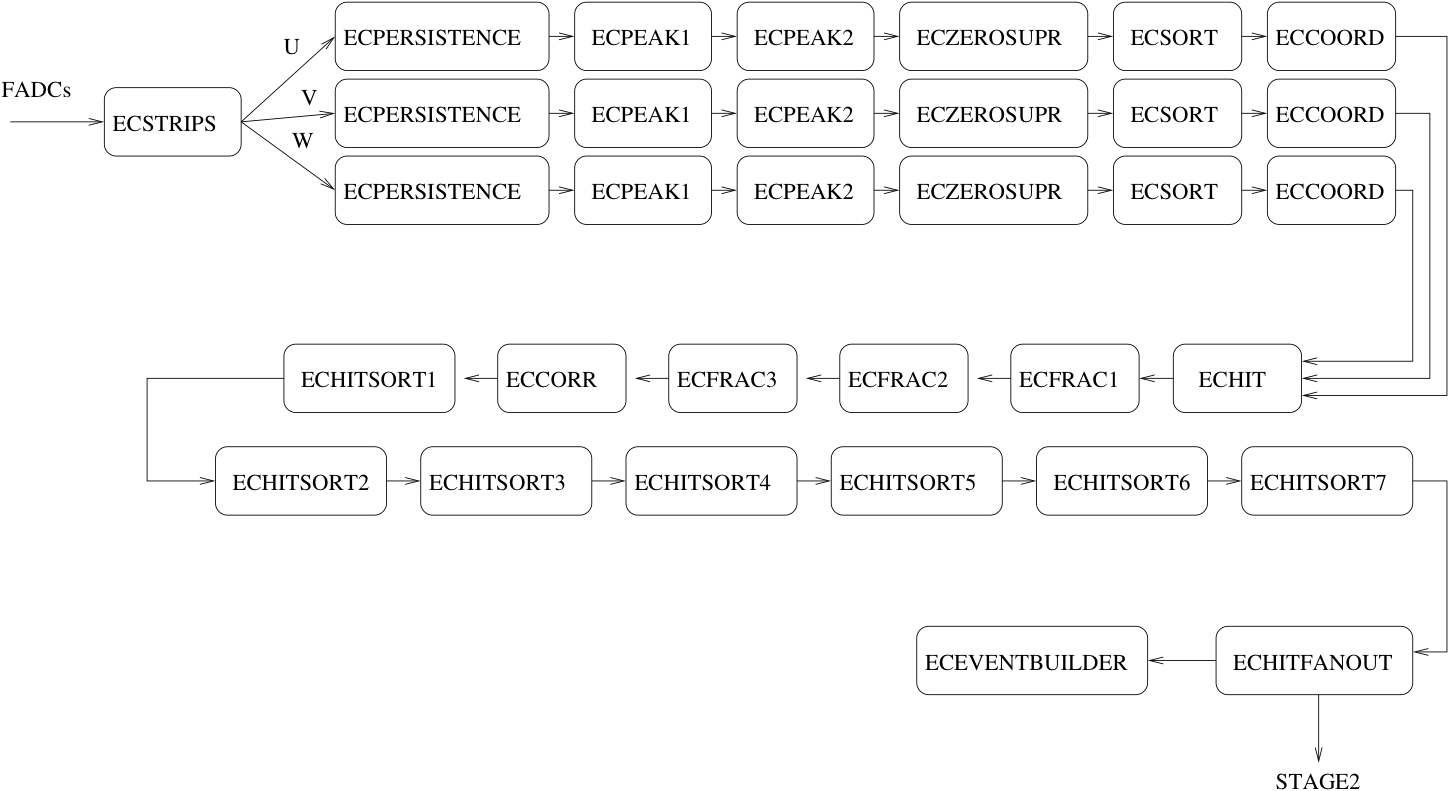
\includegraphics[width=1.0\columnwidth,keepaspectratio]{img/hls_chart.png}
	\caption{ECAL HLS project chart}
	\label{fig:hls_chart}
\end{figure}


\subsection{HLS versions and cross-project dependences}

As it mentioned before splitting project on smaller pieces allowed us to meet timing. It worked in particular because we were able to eliminate combinatorial paths between HLS projects connected by streams. Such dependence can be clearly seen looking into schematic for failed timing chains, and usually related to the large state machine control signals going between modules. Initially we were using HLS version 2015, and inspite of all our efforts we could not eliminate these long combinatorial paths across modules. This was resolved after switching to HLS version 2017 where streams could be fully registered (with pragma ‘axis register both port=‘). This meant that if registered HLS streams were used between separate HLS projects then the state machines paths were also registered between modules. With that, it was only a matter of splitting projects on smaller pieces to improve/meet timing.


\subsection{HLS Settings}

Clock uncertainty is set as 30\% of main clock, we found that it forces HLS to produce more realistic timing estimates. A single HLS project often cannot exceed several percent of FF and LUT budget, otherwise it may be a problem to meet timing requirement on VIVADO implementation step. Typical HLS project for one of the PCAL trigger elements is shown on Fig. ~\ref{fig:hls}.

\begin{figure}[hbt]
	\centering
	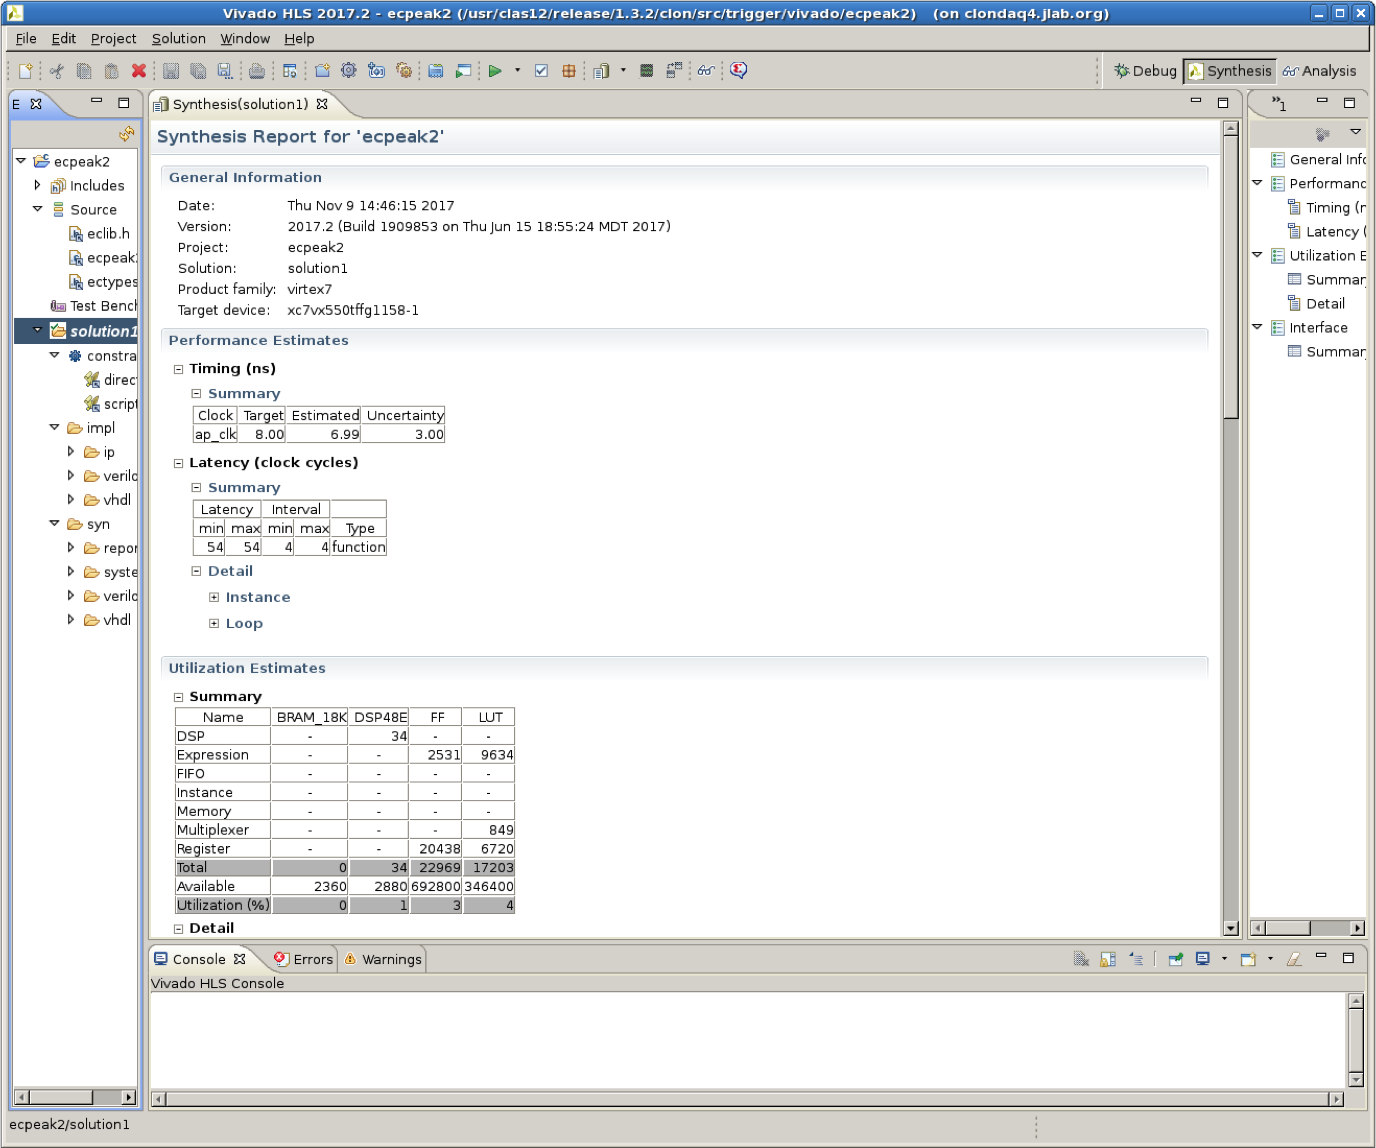
\includegraphics[width=1.0\columnwidth,keepaspectratio]{img/hls.png}
	\caption{Typical HLS project for one of the ECAL trigger elements}
	\label{fig:hls}
\end{figure}

\subsection{VIVADO Settings}

Common settings were used as shown on Fig. ~\ref{fig:vivado}. It usually takes 3+ hours to compile ECAL  project on Dell R730 server under RHEL7. For some firmware versions, we were able to utilize 100\% of LUTs and still meet timing – if clock domain was 125MHz or lower. VIVADO project for PCAL trigger is shown on Fig. ~\ref{fig:vivado}.

\begin{figure}[hbt]
	\centering
	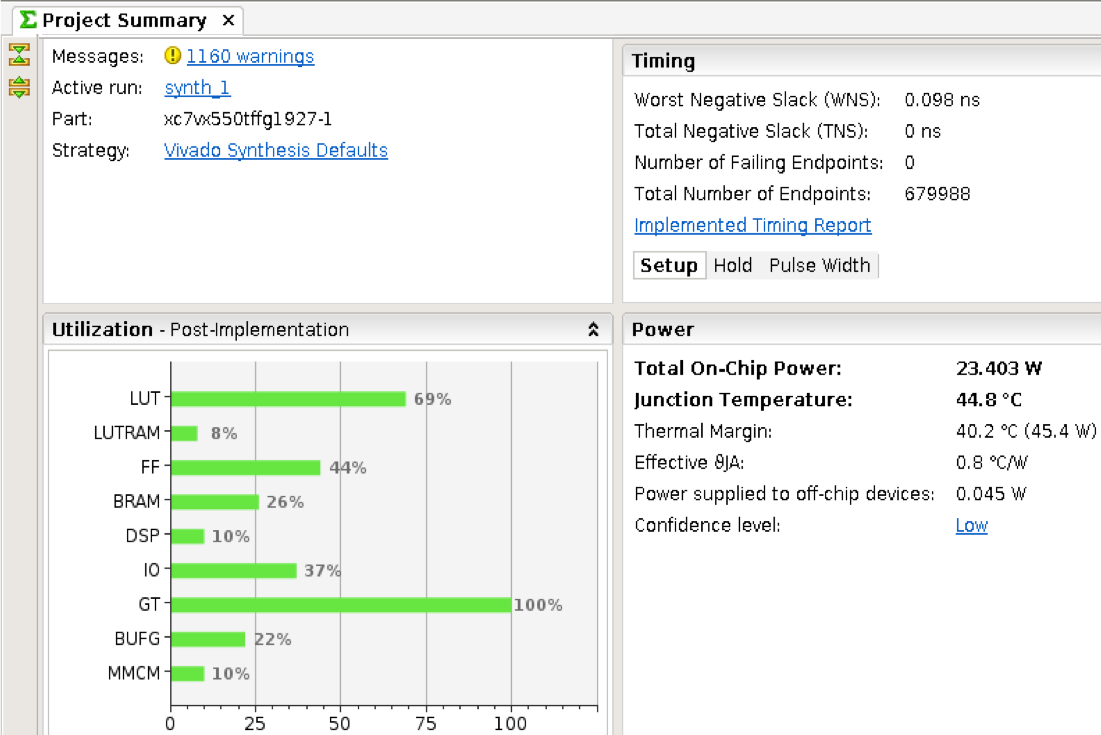
\includegraphics[width=1.0\columnwidth,keepaspectratio]{img/vivado.png}
	\caption{VIVADO project for ECAL trigger}
	\label{fig:vivado}
\end{figure}

\subsection{Firmware validation for HLS-based projects}

The ability to validate firmware using C++ implementation is the one of the biggest advantages of HLS. During the course of development and commissioning we ran HLS C++ code on simulated and real data from CLAS12 detectors, implementing required features and fixing bugs. During data taking we were able to find and fix observed problems or add new features in several hours, which was very important to save beam time.

\subsection{Our conclusion about HLS Usage}

CLAS12 ECAL and other detectors were successfully implemented into trigger system using HLS to produce core part of the firmware. This trigger was used in the first physics run and worked as expected. We were able to select events based on individual cluster energy, something which was possible before only during offline data processing.

HLS in general appears to be a useful tool, especially to implement smaller trigger components like Cherenkov or time-of-flight counters. For components utilizing significant portion of the FPGA, it will be great to improve HLS in following directions:

\begin{itemize}
	\item Support multi-clock domains
	\item Improve subroutine calls by allowing option to fully registered paths between modules. 
	\item Improve state machine logic, for example support streams between routines inside the project and be able to generate separate state machines for separate routines. It will allows to avoid splitting project manually and use HDL as top interface as we are currently forced to do.
\end{itemize}
